\documentclass[11pt]{article}
\usepackage[margin=1.5in]{geometry}
\usepackage{amsmath}
\usepackage{amssymb}
\usepackage{amsbsy}
\usepackage{bbm}
\usepackage{url}
\usepackage{color}
\usepackage{float}
\usepackage{graphicx}
\usepackage{epstopdf}
\usepackage{fancyhdr}
\usepackage{enumerate}
\usepackage{tikz}
\usepackage[ruled,vlined]{algorithm2e}
\usepackage[colorlinks=true,urlcolor=blue]{hyperref}
\usepackage[utf8]{inputenc}


\title{CS224W Homework 3}
\author{yeeboxie}

\newcommand{\Solution}[1]{{\medskip \color{red} \bf $\bigstar$~\sf \textbf{Solution}~$\bigstar$ \sf #1 } \bigskip}

\begin{document}

\maketitle
\section{GraphRNN [20 points]}

In class, we covered GraphRNN, a generative model for graph structures. Here we assume that the graph has no node types/features, and no edge types/features.

\subsection{Edge-level RNN [12 points]}
Remember that GraphRNN uses random BFS ordering to generate graphs by
iteratively adding a node and predicting its connectivity to the nodes already in the graph. Suppose that the GraphRNN model is generating a grid graph:
\begin{figure}[H]
    \centering
    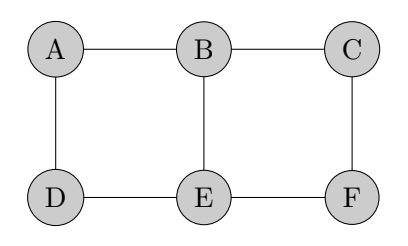
\includegraphics[width=0.4\textwidth]{CS224W_Homework3/hw3-q1.jpg}
    \caption{GraphRNN grid graph.}
\end{figure}
If we wanted a GraphRNN to generate this graph, what predictions would each cell in the edge-level RNN need to make? Recall that a GraphRNN needs to predict, for each new node, which existing nodes it needs to wire an edge with. It outputs 1 when there should be an edge, and 0 when there should not. Nodes are added in BFS ordering starting from Node A. Assume that the neighbors of a node are explored in alphabetical order (i.e. ties are broken using alphabetical ordering).

\vspace{10pt}


\noindent Sample answer format (at a particular step of the node-level RNN):


Decodes node $<\text{node\_Id}>$ (edge-level RNN predicts $<\text{edge\_value(s)}>$ for connectivity to $<\text{node\_Id(s)}>$ )\\

*fill-in $<\text{node\_Id}>$, $<\text{edge\_value(s)}>$, and $<\text{node\_Id(s)}>$\\
\\
\Solution{}

\begin{itemize}
    \item \textbf{Node B}: Decodes node B (edge-level RNN predicts [1] for connectivity to [A])
    \item \textbf{Node C}: Decodes node C (edge-level RNN predicts [0, 1] for connectivity to [A, B])
    \item \textbf{Node D}: Decodes node D (edge-level RNN predicts [1, 0, 0] for connectivity to [A, B, C])
    \item \textbf{Node E}: Decodes node E (edge-level RNN predicts [0, 1, 0, 1] for connectivity to [A, B, C, D])
    \item \textbf{Node F}: Decodes node F (edge-level RNN predicts [0, 0, 1, 0, 1] for connectivity to [A, B, C, D, E])
\end{itemize}

\subsection{Advantages of BFS ordering [8 points]}
Explain 2 advantages of graph generation with random BFS ordering of nodes in
the graph, as opposed to generating with a random ordering of nodes in the graph.\\
\\
\Solution{}

\begin{enumerate}
    \item \textbf{Captures Local Graph Structure Better}
BFS ordering tends to visit nodes that are neighbors or in the same local neighborhood before moving further away. This helps the model learn and generate more realistic local substructures (e.g., communities, clusters) as it maintains the local connectivity patterns present in real-world graphs.
    \item \textbf{Improved Dependency Modeling for Sequential Generation}
When generating graphs sequentially, BFS ordering reduces the long-range dependencies compared to a fully random ordering. Since BFS typically generates nodes that are closer in the graph structure, the RNN or generation model only needs to focus on predicting edges within a smaller, more local context, which simplifies learning and often leads to better performance.
\end{enumerate}

\section{LightGCN [25 points]}

We learned in class about \textbf{LightGCN}, a GNN model for recommender systems. Given a bipartite user-item graph $G = (V, E)$, let $\mathbf{A} \in \mathbb{R}^{|V| \times |V|}$ be its unnormalized adjacency matrix, $\mathbf{D} \in \mathbb{R}^{|V| \times |V|}$ be its degree matrix and $\mathbf{E}^{(k)} \in \mathbb{R}^{|V| \times d}$ be its node embedding matrix at layer $k$ where $d$ is the embedding dimension. Let $\tilde{\mathbf{A}} = \mathbf{D}^{-1/2} \mathbf{A} \mathbf{D}^{-1/2}$ be the normalized adjacency matrix.\\

\noindent The original GCN updates node embeddings across layers according to $\mathbf{E}^{(k+1)} = \text{ReLU}(\tilde{\mathbf{A}} \mathbf{E}^{(k)} \mathbf{W}^{(k)})$, while LightGCN removes the non-linearity and uses the equation for each layer $k\in \{0, 1, ..., K-1\}$:
\begin{equation}
    \mathbf{E}^{(k+1)} = \tilde{\mathbf{A}} \mathbf{E}^{(k)}
\end{equation}
Moreover, LightGCN adopts multi-scale diffusion to compute the final node embeddings for link prediction, averaging across layers:
\begin{equation}\label{eq:lightgcn-diff}
    \mathbf{E} = \sum_{i=0}^{K} \alpha_{i} \mathbf{E}^{(i)},
\end{equation}
where we have uniform coefficients $\alpha_{i} = \frac{1}{K + 1}$.


\subsection{Advantages of Average Embeddings [4 points]}
    Why does LightGCN average over layer embeddings? What benefits does it bring, in a recommendation systems setting?

    \textbf{What to submit?} 1-3 sentences of explanation on the reasons and benefits of averaging across layers.

    \Solution{}

\textbf{Focus on Structural Information Instead of Feature Learning}
In GCN, each layer typically learns higher-order neighborhood information by iteratively aggregating neighboring node features. However, in many cases, especially for recommendation systems, the task may not require capturing very deep graph structures (e.g., distant neighbors) but instead focuses on local structural information. Averaging embeddings across all layers helps balance this by allowing the model to capture different levels of neighborhood information (from shallow to deeper layers), rather than focusing heavily on the deeper or high-order convolutions.

By simply averaging these embeddings, the model can take advantage of the information captured at different graph depths, and use it in a more generalizable and robust way.


\subsection{Self-connection [4 points]}
We denote the embedding of an item $i$ at layer-k $\mathbf{e}_i^{(k)}$ and that of a user $u$ $\mathbf{e}_u^{(k)}$. The graph convolution operation (a.k.a., propagation rule) in LightGCN is defined as:
$$\mathbf{e}^{(k+1)}_u = \sum_{i\in\mathcal{N}_u}\frac{1}{\sqrt{\lvert\mathcal{N}_u\rvert}\sqrt{\lvert\mathcal{N}_i\rvert}}\mathbf{e}^{(k)}_i$$
$$\mathbf{e}^{(k+1)}_i = \sum_{u\in\mathcal{N}_i}\frac{1}{\sqrt{\lvert\mathcal{N}_i\rvert}\sqrt{\lvert\mathcal{N}_u\rvert}}\mathbf{e}^{(k)}_u$$  
The symmetric normalization term$\frac{1}{\sqrt{\lvert\mathcal{N}_u\rvert}\sqrt{\lvert\mathcal{N}_i\rvert}}$follows the design of standard GCN, which can avoid the scale of embeddings increasing with graph convolution operations.\\ 

\noindent However, from the equations above, we can find that in LGCN, we only aggregate the connected neighbors and do not integrate the target node itself (i.e., there is no \textbf{self-connection}). This is different from most existing graph convolution operations that typically aggregate extended neighbors and also specifically handle self-connection.\\

\noindent Does LightGCN contain implicit self-connection? If your answer is yes, which operation captures the same effect as self-connection? If no, what do you think is the reason why LightGCN doesn't need self-connection or similar effects?

\textbf{What to submit?} Yes or no and 1-2 sentences of justification.

\Solution{}

Yes, LightGCN does contain implicit self-connection despite not explicitly adding self-loops in the graph convolution equations.The symmetric normalization term effectively normalizes the neighbor embeddings, keeping the scale of embeddings stable throughout the graph convolutions.

While there is no direct self-connection (i.e., no explicit term ${e}^{(k)}$ likein the equation for the update of ${e}^{(k+1)}$ , the self-connection effect is implicitly captured by averaging the embeddings across multiple layers. In this way, the node's own embedding still contributes to the final learned representation, since higher-layer embeddings are combinations of the node's own neighbors (including itself in higher layers if it influences its neighbors in a loop).



 \subsection{Relation with APPNP [5 points]}
There is a work that connects GCN with Personalized PageRank, where the authors propose a GCN variant named APPNP that can propagate long range without the risk of oversmoothing. Inspired by the teleport design in Personalized PageRank, APPNP complements each propagation layer with the starting features (i.e., the 0-th layer embeddings), which can balance the need of preserving locality (i.e., staying close to the root node to alleviate oversmoothing) and leveraging the information from a large neighborhood. The propagation layer in APPNP is defined as:
$$\mathbf{E}^{(k+1)} = \beta\mathbf{E}^{(0)}+(1-\beta)\tilde{\mathbf{A}}E^{(k)}$$
where $\beta$ is called the ``teleport probability'' to control the retention of starting features in the propagation, and $\tilde{\mathbf{A}}$ denotes the normalized adjacency matrix.\\

\noindent Aligning with Equation (\ref{eq:lightgcn-diff}), we can see that by setting $\alpha_k$ accordingly, LightGCN can fully recover the prediction embedding
used by APPNP. As such, LightGCN shares the strength of APPNP in combating oversmoothing — by setting the $\alpha$ properly, LightGCN allows using a large K for long-range modeling with controllable oversmoothing.\\

\noindent Express the layer-$K$ embeddings $\mathbf{E}^{(K)}$ of APPNP as a function of the initial embeddings $\mathbf{E}^{(0)}$ and the normalized adjacency matrix $\tilde{\mathbf{A}}$. Show all work.

 \textbf{What to submit?} Multi-line mathematical derivation of the relationship between $\mathbf{E}^{(K)}$ and $\mathbf{E}^{(0)}$

\Solution{}
\begin{align}
    \numberwithin{equation}{section} % Reset equation numbering within the section
    \setcounter{equation}{0} % Start numbering from 1 for this block
    \mathbf{E}^{(k+1)} &= \beta \mathbf{E}^{(0)} + (1-\beta) \tilde{\mathbf{A}} \mathbf{E}^{(k)} \\
    \mathbf{E}^{(0)} &= \mathbf{E}^{(0)} \\
    \mathbf{E}^{(1)} &= \beta \mathbf{E}^{(0)} + (1-\beta) \tilde{\mathbf{A}} \mathbf{E}^{(0)} \\
    \mathbf{E}^{(2)} &= \beta \mathbf{E}^{(0)} + (1-\beta) \tilde{\mathbf{A}} \mathbf{E}^{(1)}= \beta \mathbf{E}^{(0)} + (1-\beta) \tilde{\mathbf{A}} \left( \beta \mathbf{E}^{(0)} + (1-\beta) \tilde{\mathbf{A}} \mathbf{E}^{(0)} \right) \\
    \mathbf{E}^{(2)} &= \beta \mathbf{E}^{(0)} + (1-\beta) \beta \tilde{\mathbf{A}} \mathbf{E}^{(0)} + (1-\beta)^2 \tilde{\mathbf{A}}^2 \mathbf{E}^{(0)} \\
    \mathbf{E}^{(k)} &= \beta \mathbf{E}^{(0)} + (1-\beta) \tilde{\mathbf{A}} \mathbf{E}^{(k-1)} \\
    \mathbf{E}^{(k)} &= \beta \mathbf{E}^{(0)} + (1-\beta) \tilde{\mathbf{A}} \beta \mathbf{E}^{(0)} + (1-\beta)^2 \tilde{\mathbf{A}}^2 \mathbf{E}^{(0)} + \dots + (1-\beta)^{k-1} \tilde{\mathbf{A}}^{k-1} \mathbf{E}^{(0)} \\
    \mathbf{E}^{(K)} &= \sum_{i=0}^{K-1} (1-\beta)^i \tilde{\mathbf{A}}^i \mathbf{E}^{(0)} + \beta \mathbf{E}^{(0)}
\end{align}


 
    \subsection{Recommendation Task [12 points]}%need to change
     We are given the following bipartite graph. Solid edges represent already-observed user-item interactions, while dotted edges denote the set of positive interactions \emph{in the future}.
    \begin{center}
    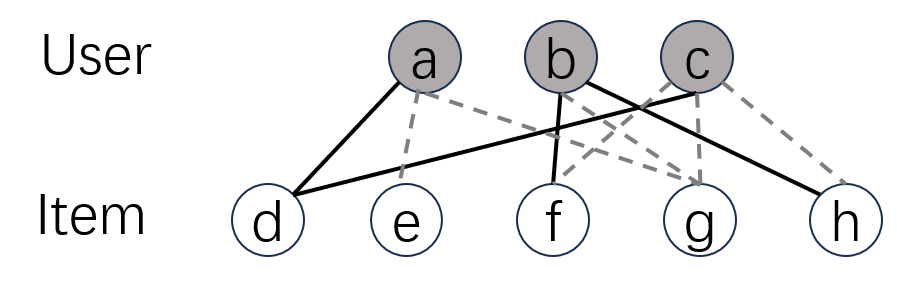
\includegraphics[scale = 0.35]{CS224W_Homework3/3.4.png}
    \end{center}
    One-dimensional embeddings for the nodes are listed in the following table.
    \begin{center}
    \begin{tabular}{|c|c|c|c|c|c|c|c|}
    \hline
    a & b & c & d & e & f & g & h\\ [0.5ex]
    \hline
    0.3 & 0.96 & 0.7 & 0.6 & 0.4 & 0.8 & 0.7 & 0.64 \\
    \hline
    \end{tabular}
    \end{center}
    We are given a recommendation model that uses L2 distance (lower distance means higher recommendation) between user and item embeddings to calculate the scores.\\

    \noindent Compute the Recall@2 score for users $a, b, c$. For each user, explicitly write out the positive items $P_{u}$ and recommended items $R_{u}$, as sets of the form $\{ X,Y,Z \}$. Please exclude already-interacted items in $R_{u}$, as we are only interested in recommending not-yet-interacted items.\\

    \noindent Fill in your answers in the following table. Where the first 5 columns represent user-item distances. What is the final Recall@2?
    \vspace{0.5cm}
    
    $\begin{bmatrix}
      & d & e & f & g & h & P_{u} & R_{u} & \text{Recall@2} \\
    a &  & &  &  &  &  & &  \\
    b &  &  &  & &  & &  &  \\
    c &  &  &  &  &  & & &
    \end{bmatrix}$
    \vspace{0.5cm}
    
    \textbf{What to submit?} The $P_{u}$, $R_{u}$, and the Recall@2 values for each of the users, as well as the overall final Recall@2.

    \Solution{}

    $\begin{bmatrix}
    & d & e & f & g & h & P_{u} & R_{u} & \text{Recall@2} \\
    a & 0.3  & 0.1 & 0.5  & 0.4  & 0.34  & $\{ e,g \}$ & $\{ e,h \}$ & $0.5$  \\
    b & 0.36  & 0.56  & 0.16  & 0.26 & 0.32  & $\{ g \}$ & $\{ d,g \}$  & $1.0$  \\
    c & 0.1  & 0.3  & 0.1  & 0  & 0.06  &$\{ f,g,h \}$ &$\{ g,h \}$ & $1.0$ \\
      & & & & & & & & $0.83$
    \end{bmatrix}$
 

\section{Honor Code [0 points]}
(X) I have read and understood Stanford Honor Code before I submitted my
work.

**Collaboration: Write down the names \& SUNetIDs of students you collaborated with on Homework 2 (None if you didn’t).**

**Note: Read our website on our policy about collaboration!**

\end{document}
